\documentclass[fleqn,10pt]{wlscirep}
\usepackage[utf8]{inputenc}
\usepackage[T1]{fontenc}
\usepackage{ucs}
\usepackage{subcaption} 
\usepackage{tabularx}
\usepackage[font=small,labelfont=bf,tableposition=top]{caption}
\usepackage{todonotes}
\usepackage[draft]{pgf}

\newcommand{\executeiffilenewer}[3]{%
  \ifnum\pdfstrcmp{\pdffilemoddate{#1}}%
  {\pdffilemoddate{#2}}>0%
  {\immediate\write18{#3}}\fi%
}
% set inkscape binary path according to operating-system
\IfFileExists{/dev/null}{%
  \newcommand{\Inkscape}{inkscape }%
  }{%
  \newcommand{\Inkscape}{"C:/Program Files/Inkscape/inkscape.exe" }%
}
% includesvg[scale]{file} command
\newcommand{\includesvg}[3][1]{%
  \executeiffilenewer{#2.svg}{#2.pdf}{%
  \Inkscape -z -D --file="#2.svg" --export-pdf="#2.pdf"}%
  \scalebox{#1}{\includegraphics[width=#3\textwidth]{#2.pdf}}%
}

\title{VIST – A Variant-Information Search Tool for Precision Oncology}

\author[1]{Jurica Ševa}
\author[3]{Julian G\"otze}
\author[2]{Mario Lampping}
\author[2,4,5]{Damian Rieke}
\author[2]{Reinhold Sch\"afer}
\author[1]{Patrick Jähnichen}
\author[1]{Madeleine Kittner}
\author[1]{Steffen Pallarz}
\author[1]{Johannes Starlinger}
\author[1,*]{Ulf Leser}

\affil[1]{Knowledge Management in Bioinformatics, Department of Computer Science, Humboldt-Universit\"at zu Berlin, Rudower Chaussee 25, 12489 Berlin, Germany}
\affil[2]{Charité Comprehensive Cancer Center, Charit\'eplatz 1, 10117 Berlin, Germany}
\affil[3]{University Hospital T\"ubingen, Hoppe-Seyler-Straße 3, 72076 Tübingen, Germany}
\affil[4]{Department of Hematology and Medical Oncology, Campus Benjamin Franklin, Charit\'e Unviersit\"atsmedizin Berlin, Hindenburgdamm 30, 12203 Berlin, Germany}
\affil[5]{Berlin Institute of Health (BIH), Kapelle-Ufer 2, 10117 Berlin, Germany}
\affil[*]{leser@informatik.hu-berlin.de}

\keywords{Clinical Relevance, Document Retrieval,Personalized Oncology,Precision Oncology,Variants NER,Genes NER,Document Classification,Machine Learning,Web Interface,Document Triage}

\begin{abstract}
Diagnosis and treatment decisions in cancer increasingly depend on a detailed analysis of the mutational status of a patient’s genome. This analysis in turn relies on previously published information regarding the association of variations to disease progression and possible interventions. Clinicians to a large degree use biomedical search engines to obtain such information; however, the vast majority of search results 
%in the common search engines 
focus on basic science and are clinically irrelevant. 
We developed the Variant-Information Search Tool (VIST), a search engine designed for the targeted search of clinically relevant publications given a mutation profile. 
VIST indexes all PubMed abstract, applies advanced text mining to identify mentions of genes, variants and chemicals/drugs and uses machine-learning based scoring to judge the (clinical) relevancy of documents. 
Its functionality is available through a fast and intuitive web interface. 
We performed several evaluations, showing that VIST’s ranking is superior to that of PubMed or a pure vector space model.
The results of this work are several: 1) an initial investigations of clinical relevance, focusing on precision medicine, with supporting trained machine learning classification models, 2) a manually/expert annotated gold standard corpus for clinical relevance, 3) a et of real life queries with supporting PubMed publications, 4) an Web application, which serves as a search engine, annotation tool and evaluation tool.
\end{abstract}
\begin{document}

\flushbottom
\maketitle
% * <john.hammersley@gmail.com> 2015-02-09T12:07:31.197Z:
%
%  Click the title above to edit the author information and abstract
%
\thispagestyle{empty}

%\noindent Please note: Abbreviations should be introduced at the first mention in the main text – no abbreviations lists. Suggested structure of main text (not enforced) is provided below.

\section*{Introduction}
Precision oncology denotes treatment schemes in cancer in which medical decisions depend on the individual molecular status of a patient \cite{Garraway2013}. 
The most relevant molecular information is the patient’s genome, or, more precisely, the set of variations (mutations) each individual carries. 
Today a number of diagnosis and treatment options already depend on the (non-)existence of certain variations in a tumor \cite{Topalian2016}. 
When faced with the variant profile of a patient, clinicians critically depend on accurate, up-to-date, and detailed information regarding the clinical relevance of the present variations. Finding such information is highly laborious and time-consuming, often taking hours or even days \cite{Doig2017}. 
Clinicians use multiple search engines, such as PubMed, clinicaltrials.gov, or asco.org, and multiple databases, such as Cosmic \cite{Forbes2015}, DrugBank \cite{Wishart2008}, or Ensemble \cite{Varadi2015}. 
Especially important are specialized databases providing manually curated evidences for variation-therapy associations, such as OncoKB \cite{Chakravarty2017}, ClinVar \cite{Landrum2016}, or CIViC \cite{Griffith2017}. 
We report on VIST, a search engine specifically developed to aid clinicians in precision oncology in their search for clinically relevant information for a (set of) variations or mutated genes. 
As such it was developed to support the inner workings of a tumor board which goal is to determine the best possible cancer treatment and care plan for an individual patient.
As for any search engine, the core of VIST is its ranking function which, given a (set of) variation or a (set of) gene and a cancer entity, ranks those documents of its corpus highest which contain clinically relevant information. The main difficulty when developing a ranking function for such a novel and quickly emerging field are (a) the lack of gold standard data and (b) the complexity of the concept "clinical relevance", which encompasses information about gene-mutation-drug associations, frequencies of variations within populations, clinical trials, mode of action of drugs, molecular functions and pathways associated with a variation, reports on treatments of similar tumors, etc. When developing VIST we took two measures to cope with this complexity: (1) We use advanced information extraction to pre-filter documents based on the genes and variations they mention, and we (2) developed a document classifier using a silver-standard corpus of clinically related documents obtained from two different sources. VIST furthermore offers several metadata filters (journal, year of publication), highlights key phrases (i.e., the clinically most important sentences) and mentions of query entities when displaying documents, links out to external databases, and allows mixing of entity and classical keyword search. Furthermore, we performed a user study to obtain a set of <query, document, relevance> triples which allows for a systematic comparison to other search engines, showing that VIST’s ranking outperforms that of PubMed and a pure vector space model (VSM) in most cases. VIST was developed in close interaction with medical experts and is freely available at https://triage.informatik.huberlin.de:8080/

%\section*{Related work}
There are a number of search engines specialized for biomedical applications, but none that focuses specifically on precision oncology and clinical relevance. The most popular engine, PubMed, essentially search ranks results by the date of publication \cite{Fiorini2017}. Tools like GeneView \cite{Thomas2012}, PubTator \cite{Wei2013a} or SemeDa \cite{Kohler2003} pre-annotate documents in their index using various Named Entity Recognition (NER) tools to allow searching across spelling variations and synonyms. They also highlight recognized entities in matching documents. DigSee \cite{Kim2013} performs keyphrase detection for sentences describing the relationship between genes and diseases. DeepLife \cite{Ernst} also performs entity recognition and, in contrast to the previous tools which all consider only PubMed abstracts, also indexes certain web sites and social media content. RefMED \cite{Yu2009} facilitates search in PubMed by user relevance feedback. In contrast to VIST, none of these tools ranks according to a specific thematic focus of documents.

There are also a few search tools which are topically closer to VIST. The Cancer Hallmarks Analytics Tool (CHAT) \cite{Baker2017} classifies literature based on the predefined cancer hallmarks taxonomy. ASCOT \cite{Korkontzelos2012} searches texts in clinical trials, but has no cancer focus and does not apply advanced information extraction to find genes or variations. DGIdb \cite{Cotto2017} offers search over a database of text-mined clinically relevant drug-gene pairs; in contrast, VIST returns entire documents and has a much wider scope than just drug-gene pairs. A valuable recent contribution is the TREC Precision Medicine Track \cite{Roberts2017}, started in 2017 (and available again this year). INCORPORATE RELEVANT BIONLP/ACL PAPERS (\cite{W18-2313}, \cite{W18-2310}, \cite{seva2018}). 


\input{sections/related.tex}

\section*{Results}
VIST was extensively evaluated to assess and optimize its performance. First, we used a prototype version of VIST to curate a new corpus of clinically (ir-)relevant documents for performing evaluations (Section 4.1). We assessed the accuracy of the clinical-relevance classifier on this data set using CV (Section 4.2). Finally, we used this set to compare the ranking performance of VIST with that of PubMed and a pure VSM (Section 4.3).

\subsection*{Evaluated Ranking Functions}

\begin{table}[]
\begin{tabularx}{\textwidth}{|l|X|}
\toprule
\textbf{Ranking function} & \textbf{Ranked by:} \\ \midrule
\textit{confidence\_is DESC} & cancer-related classifier score. \\ \midrule
\textit{confidence\_is DESC, pubdate DESC} & cancer-related classifier score. Rank documents with matching cancer-related classifier score by their publication date. \\ \midrule
\textit{score desc} & Solr search score. \\ \midrule
\textit{product(pubdate,confidence\_is) desc} & product of publication date and cancer-related classifier score. \\ \midrule
\textit{score desc, confidence\_is desc, pubdate desc} & Solr search score. Rank documents with matching Solr search score by cancer-related classifier score. Rank documents with matching Solr search score and cancer-related classifier score by their publication date. \\ \midrule
\textit{product(query(\$q),confidence\_is) desc} & product of Solr search score and cancer-related classifier \\ \midrule
\textit{linear regression} & linear regression \\ \bottomrule
\end{tabularx}
\caption{Implemented ranking functions: CHANGE THE NAMES OF RANKINGS (i.e. use wildcards or something)}
\label{tab:rankingFunctions}
\end{table}

% \begin{figure}[htbp]
% \begin{minipage}[b]{0.5\linewidth}
% \centering
% 	\includesvg{img/eval/SearchSortCombined}{1}
% 	\caption{VIST: evaluation of implemented ranking functions and search strategies. RESULTS FOR VIST1 (NO CLINICAL RELEVANCE CLASSIFICATION)! ADD VIST2 TO THE GRAPH WITH SAME QUERY FUNCTIONS. ADD query(\$q) TO BOTH VERSIONS. LABEL 1 - N INSTEAD OF TEXT TO SAVE SPACE.}
% 	\label{img:searchSort}
% \end{minipage}
% \hspace{0.5cm}
% \begin{minipage}[b]{0.5\linewidth}
%       \centering
% 	\includesvg{img/eval/VISTErrorIssues}{1}
% 	\caption{VIST: Document retrieval error causes.}
% 	\label{img:vistErrors}
% \end{minipage}
% \end{figure}

\missingfigure{Testing a long text string}

First, we focused on determining the optimal search strategy. For this we tried out four different search strategies: \textit{exact match}, where returned documents had to match the search queries,  \textit{ \~{ } (or fuzzy) strategies}, with an allowed string distance of 1 or 2, respectively, against the original search terms and \textit{expanded search}, where the original query terms were expanded with known synonyms of gene names. The known synonyms where obtained from an integrated knowledge database, developed in our research group but as of yet not publicly available. As seen in Figure \ref{img:searchSort}, the best performing search strategy is \textit{expanded search}. The other three evaluated search strategies obtained significantly lower results (approx. 10\%). 

%In addition to the overall performance of VIST, 
Additionally, we also focused on the positions where CIViC PMIDs are found among the returned documents. To evaluate this, we implemented 6 different ranking functions, by using various metadata stored in the Solr index. 
The evaluated ranking functions and respective descriptions are given in Table \ref{tab:rankingFunctions}.
%VIST additionally ranks returned documents against the input query. 
%The number of possible candidates for the ranking function, as well as their combinations, is high. 
%For that we developed six ranking functions, evaluated against the documents from CIViC data set. 
The goal of the ranking function is to optimize the positioning of relevant documents in the returned document list. 
%based on the number of returned and missed documents, as available in the CIViC data set. 
The evaluation shows%, as seen in Figure \ref{img:searchSort} (left), 
that the classification score, obtained from the cancer-related classification model, plays a significant role in the ranking scheme. 
%as the ranking functions which do not use that score perform worse than the ones which include that score. 
As the best performing ranking function a product of the cancer-related classification score and the internal Solr score was determined. 
%Additionally, another important information is not only the number of retrieved documents but also their positioning in the list of ranked returned documents. in both cases higher is better. 

%\begin{figure}[t]
%\centering
%	  \includesvg{img/eval/SortFunctionsSummaryBokehAlternative}{1}
%\caption{VIST: evaluation of ranking functions - REDO AS LINE GRAPH, USING ONLY DATA FROM BEST PERFORMING ML MODEL AND EXPANDED SEARCH STRATEGY!}
%\label{img:sortStrategies}
%\end{figure}

%\begin{figure}[t]
%\centering
%		\includesvg{img/eval/CIViCPositionDistribution}{1}
%		\caption{Distribution of CIViC document positions in search results}
%\label{img:journalSelectionEffect}
%\end{figure}
%
%Furthermore, we were also interested in the effect developed filters have on the search performance. For that evaluated various combinations of publication years range (1988-2017, 2005-2017 and 2010-2017 respectively) as well as a selection of desired journals (all journals, all CIViC journals as well as top 20, top 10 and top 5 journals from the CIViC dataset). The results of this evaluation are shown in Figure \ref{img:journalSelectionEffect}. We see that the distribution resembles a Zipf distribution. This means that most relevant documents do appear in the top 100 returned documents.

As seen from the Figure \ref{img:searchSort}, it is clear that VIST does not find all documents from CIViC. As this is a potentially big issue for the performance of the system, we investigated the main causes for this behaviour. This evaluation was performed by manually analysing 46 documents from various queries, which were not found by VIST. The results of this evaluation are shown in Figure \ref{img:vistErrors}. The main detected issues were of a technical nature: the search term(s) were either not present in the abstract of the missed scientific publication, the abstract was missing from the VIST Solr index due to parsing issues or the search term was not recognized by the used NER tools.

\subsection*{User Evaluation}
To obtain a fresh set of clinically relevant (or not) documents for evaluating our models, we performed a user evaluation encompassing four medical experts. We gathered a set of 20 queries each consisting of a gene or a variation which occurred in recent real treatment situations at the Charitè clinic. For each query, we used Solr default ranking to find (up to) 10 matching publications. Next, each of the four experts assessed the clinical relevancy (using a 5-point Likert scale) of each returned document given the query, resulting in a set of 188 triples <query, document, score>. Assessment showed a low degree of agreement at the 5-point scale (40\% of all pairwise assessments agree), but better agreement when aggregated to binary decision (62\% agreement). To obtain a robust evaluation set, we (1) removed all pairs <query, document> which were assessed as "highly relevant" but at least one expert and as "not relevant at all" by at least one other expert and (2) obtained final assessments for all other pairs by majority voting. This resulted in a list of 119 <query, document> assessments, consisting of 49 relevant and 70 irrelevant pairs.

\subsection*{Performance on Test Set}
We used this manually created corpus as test set for a classifier for clinical relevance. This classifier was trained using different sets (see Section 3.2). For each set, the optimal configuration was obtained using 10-fold cross validation (CV) and evaluated on the test set. Specifically, we tested OncoKB Original, consisting only of OncoKB articles, OncoKB Balanced, where we balanced the class composition using under sampling of the majority (the negative) class, and OncoKB+CIViC, which combines OncoKB Original and CIViC. Results are shown in Table \ref{tab:vist_clinical_relevance}. 

%\begin{figure}[htbp]
%\centering
\begin{minipage}{\linewidth}
	\begin{minipage}[b]{0.5\linewidth}
	%\begin{figure}[htbp]
	%\centering
	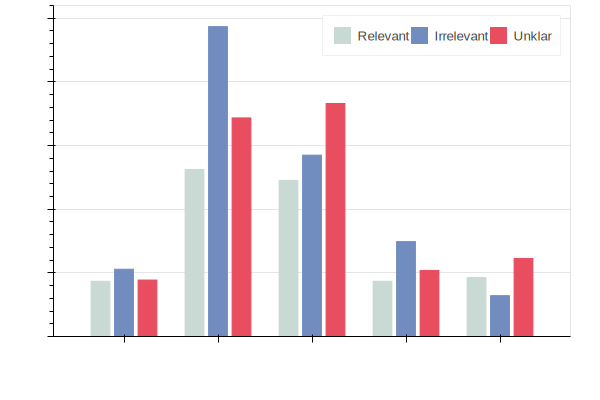
\includegraphics[width=\linewidth]{img/eval/ablationGS.png}
	\captionof{figure}{Overlap of annotated biomedical entities over the relevance group corpora. NOT MENTIONED/EXPLAINED IN TEXT: SHOWS THAT AMONG THE THREE CLASSES (RELEVANT;IRRELEVANT;UNCLEAR) THERE IS VERY LITTLE DIFFERENCE WHEN IT COMES TO THE MENTION OF 5 DIFFERENT BIO ENTITIES (CHEMS; GENES; MUTS; DISEASES; SPECIES). CONFIRMS THAT CLINICAL RELEVANCE IS HARD TO MODEL! INCREASE FONT FOR TEXT/LABELS! }
	\label{img:abelationGS}
%	\end{figure}
	\end{minipage}
	\hspace{0.3cm}
%	\hfill
	\begin{minipage}[b]{0.5\linewidth}
		\centering
%		\begin{table}[]
		\begin{tabular}{@{}|l|l|c|r|@{}}
		\toprule
		\textit{\textbf{Property}}               & \textit{\textbf{Count}} \\ \midrule
		OncoKB Balanced & Decision Tree & 0.65 & 0.65 \\ \midrule
		OncoKB + CIViC* & Linear SVM & 0.71 & 0.71 \\ \midrule
		OncoKB Original & Linear SVM & 0.66 & 0.37 \\ \midrule
		\end{tabular}
		\captionof{table}{Performance of clinical relevance models on expertgenerated test set. P: Precision on relevant class. * Model used in VIST production server.}
		\label{tab:vist_clinical_relevance}
%		\end{table}
	\end{minipage}
\end{minipage}

\subsection*{Comparison to Baselines}
We compared the ranking of VIST with that of PubMed (using Entrez E-utilities (Sayers, 2008)) and that of a plain VSM ranking using Solr. In these comparisons we cannot compare absolute ranks of results as VIST performs result filtering by entities and by cancer type, leading to much different result set sizes. Instead, we use two metrics which are robust to different result set sizes. Figure \ref{img:ranking} shows, for each query, the ratio of the average rank of all relevant documents from our test data to the average rank of all irrelevant documents. VIST performs best in 11 out of the 16 queries and very close to the best in 5 out of 16 queries. Figure \ref{img:p_r_k} im shows average precision@k and recall@k for all three systems; therein, k denotes the k’th document in the ranked result that is also contained in the test set. Clearly, VIST outperforms VSM-ranking and PubMed in both regards.

\begin{figure}[htbp]
\centering
\begin{minipage}[b]{0.45\linewidth}
	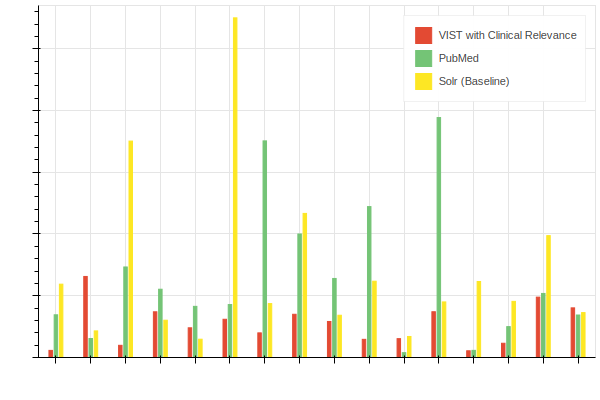
\includegraphics[width=\linewidth]{img/eval/IrRelevantPositionsRatio_baseline_bar.png}
	\caption{VIST ranking compared to PubMed and Solr. Smaller values are better. Ratios above 1 imply that irrelevant documents were on average higher ranked than relevant ones, which only once is the case for VIST.}
	\label{img:ranking}
\end{minipage}
\hspace{0.3cm}
\begin{minipage}[b]{0.45\linewidth}
	\includegraphics[width=\linewidth]{img/eval/P_R_at_K.png}
	\caption{Precision/Recall @ k averaged over all queries. Here, k denotes the k’th document in the result set that is also contained in the test set.}
	\label{img:p_r_k}
\end{minipage}
\end{figure}

ABLATION STUDY FOR WHERE VIST2 NOT BEST!
%ABLATION STUDY FOR GOLD STANDARD FROM EVAL!

\subsection*{Performance on auxiliary evaluation dataset}

Dataset generated on real life use cases over a period of 3 years. 

All PPTs deidentified/anonymized. 

Represetned (Gene, [list of PMIDs]) pairs. Possibliy extended with mutations and cancer types (omited from our queries due to VISTs suport for limited cancer types and ambiguity connected to mutations). 

No overlap between either CiVIC or OncoKB data set and this corpus.

Describe Data set Statistics!

\begin{table}
\begin{minipage}{0.5\linewidth} 

\begin{tabular}{|l|r|r|}
\hline
Metric   &   VIST & PubMed \\ \hline
Mean Average Position & $\approx$ 256 & $\approx$ 300 \\ \hline
Mean Reciprocal Rank & $\approx$0.04 & $\approx$ 0.017 \\ \hline
Mean Average Precision & $\approx$0.029 & $\approx$0.015 \\ \hline
\end{tabular}
\caption{VIST vs PubMed on the external GS data set (Marios PPTs) on top 1000 retrieved documents. Low values are due to a small number of known PMIDs for individual query. NOT MENTIONED/EXPLAINED IN TEXT!}
\label{tab:mariosGSEvaluations}

\begin{tabular}{|l|r|r|}
\hline
Metric   & Score \\ \hline
Precision & \\ \hline
Recall & \\ \hline
F-score & \\ \hline
\end{tabular}
\caption{Performance of the best performing classification model for clinical relevance on external GS data. NOT MENTIONED/EXPLAINED IN TEXT!}
\label{tab:relevanceClassifierMarioGS}

\end{minipage}
\hspace{0.5cm}
\begin{minipage}{0.5\linewidth} 
\begin{tabular}{|l|r|r|r|}
\toprule
 Position (From - To)   &   PubMed &   VIST & Both \\
\hline
 1.0 - 100.0            &    97.00 & 148.00 & - \\
 101.0 - 200.0          &    68.00 &  54.00 & - \\
 201.0 - 300.0          &    33.00 &  30.00 & - \\
 301.0 - 400.0          &    27.00 &  26.00 & - \\
 401.0 - 500.0          &    25.00 &  16.00 & - \\
 501.0 - 600.0          &    17.00 &  17.00 & - \\
 601.0 - 700.0          &    17.00 &  17.00 & - \\
 701.0 - 800.0          &    18.00 &  15.00 & - \\
 801.0 - 900.0          &    11.00 &  13.00 & - \\
 901.0 - 1000.0         &    12.00 &   9.00 & - \\
 \hline
 Sum                    &   325.00 & 345.00 & - \\
 \hline
 Nothing found		& 66 & 69 & 55 \\
\hline
\end{tabular}
\caption{Binned count of found documents in top 1000 documents over 172 distinct queries on the external GS data set (Marios PPTs). NOT MENTIONED/EXPLAINED IN TEXT!}
\label{tab:marios_bins}
\end{minipage}
\end{table}

\section*{Discussion}
We developed VIST, a search engine to support the retrieval of clinically relevant documents for precision oncology, and evaluated its performance in different manners. Despite its superior ranking performance compared to two baselines, we see a number of issues that need to be addressed in the future. First, the gold standard used for evaluation is small; we plan for a second user study then using the current VIST ranking functionality which should increase the number of relevant documents. Second, we are working to also index reports from clinicaltrials.gov. Third, we acknowledge that the current evaluation mode is rather simplistic, as it disregards the possibility to combine variant names with additional keywords to enforce clinical relevance manually, which is technically possible in all three systems we compared. Finally, we are also exploring multiple methods to improve the ranking itself.
Although the current version of the tool achieves satisfactory results, several directions for future research have opened up in the course of our work. First, as VIST
relies on the quality of developed ML models, improving current models is a viable option. In contrast to the current ML algorithms used, a more modern approach, relying on neural networks/deep learning, could be a valuable alternative. The focus of future work will shift more towards on the question of clinical relevance, as this is the focal point in the proposed application scenario. There is also the question of document classification with regards to cancer types. As the number of supported cancer types currently is limited to four (with one being an ambiguous type cancer), VIST would benefit from increasing their number . Here, as well as with determining the clinical relevance of the document, current gold standard corpora is severely biased towards a single or handful classes. This suggests that semi-supervised machine learning models could be interesting research directions with this topic. Areas such as reinforcement learning, imitation learning and few-, one- or zero-shot learning are most promising. Semi-supervised machine learning methods could be also used to improve the ranking of the matching documents. This could be tackled by relying on Learning To Rank (known also as machine-learned ranking).

In addition on improving current machine learning models, expanding the textual resources VIST analyses is a valuable future goal. Extending VIST to include publicly accessible full text articles would increase the usefulness of the tool (e.g. available over the PMC interface, with 1.6 million full text articles). Extracting structured information from full text is significantly more complex than working with smaller bodies of text (e.g. abstracts) and would, in it self, contain a new research project. Although PubMed represents the majority of freely available scientific publications, including other available resources (e.g. Clinical Trials) could expand on the usefulness of the tool. 

A final possible extension of this work looks at the possibilities of redefining ranking functions, based on the input query, its overlap with available scientific publications but also on leveraging the available information, hidden in the text, in a better way. Representing the publications as a graph is one possibility, with focus on the relationships between genes, variants and relevant diseases.
%\section*{Methods}
%
%Topical subheadings are allowed. Authors must ensure that their Methods section includes adequate experimental and characterization data necessary for others in the field to reproduce their work.

\section*{VIST: Methods}
VIST is a document retrieval system which ranks PubMed abstracts according to their clinical relevance for a (set of) variations and/or genes and a cancer entity (see Figure \ref{img:docDetails}). When inserted into the index, documents undergo a comprehensive processing pipeline including textual preprocessing, metadata extraction, named entity recognition, classification regarding cancerrelatedness, cancer type, and clinical relevance, and keyphrase detection\cite{seva2018}. Documents and their associated annotations are indexed using Solr which is also used for query processing and ranking. See Table \ref{tab:vist_index} for statistics on the corpus.

\begin{minipage}{\linewidth}
	\begin{minipage}[b]{0.45\linewidth}
	%\begin{figure}[htbp!]
	%\centering
	%\includegraphics[scale=0.3]{img/vist_preprocessing.png}
	\includegraphics[width=\linewidth]{img/vist_backend.png}    
	\captionof{figure}{VIST: Backend with preprocessing and indexing modules}
	\label{img:docDetails}
	%\end{figure}
	\end{minipage}
	\hspace{0.3cm}
%	\hfill
	\begin{minipage}[b]{0.45\linewidth}
	%\begin{table}[]
	\begin{tabular}{@{}|l|r|@{}}
	\toprule
	\textit{\textbf{Property}}               & \textit{\textbf{Count}} \\ \midrule
	Indexed documents                        & 28,401,483              \\ \midrule
	Classified as related to cancer          & 591,871                 \\ \midrule
	Classified as clinically relevant        & 5,062,340               \\ \midrule
	Clinically relevant \& cancer            & 324,033                 \\ \midrule
	Distinct variations                      & 478,656                 \\ \midrule
	Documents with \textgreater 0 variations & 314,279                 \\ \midrule
	Total number of variations               & 1,018,321               \\ \bottomrule
	\end{tabular}
	\captionof{table}{VIST Index Summary}
	\label{tab:vist_index}
	%\end{table}
	\end{minipage}
\end{minipage}

We first parse the XML format of PubMed using \cite{Achakulvisut2016} to extract metadata and main text. We detect and normalize gene mentions using GNormPlus \cite{Wei2015a} variations using tmVar\cite{Wei2013b}, and chemicals using tmChem\cite{Leaman2015}. Document classification and ranking are discussed next. 

\subsection*{Document classification for ranking}
The main purpose of VIST is to rank documents discussing the queried genes / variations according to their clinical relevance. To this end, we pre-rank all documents according to two scores: One for their relatedness to cancer in general, and one for clinical relevance. Due to lack of space, we only briefly discuss the former here, while our evaluation will focus on the latter. We use supervised document classification for both cases. All models are built using scikit-learn\cite{sklearn} and utilize tf-idf weighting. Cancer Relatedness and Cancer type. We use CIViC to build a corpus of cancer-related documents. CIViC is a cancer-oriented database of associations between human variations and phenotypes curated manually by medical experts. For cancer classification, we used all articles in CiViC as positive samples (n $\approx$ 1400) and randomly sampled abstracts from PubMed as negative samples (n $\approx$ 20,000). We trained a Logistic regression classifier using words and word-bigrams as features, achieving an accuracy of 95\% in 10-fold cross-validation (CV). As CIViC also annotates the specific cancer type of an association, we also used it to classify abstracts regarding cancer entities; due to lack of training data, we currently only distinguish melanoma, head and neck and colorectal cancer. A 10-fold CV shows an average accuracy of 0.82. Clinical Relevance. There is no simple definition of a clinically-relevant scientific publication. To circumvent this problem, we used classification based on documents curated in OncoKB, a database of similar scope as CIViC but which additionally distinguishes between clinical relevant associations (n=446) and those that are not (n=3507). Since preliminary results with this data set were very sensitive to class imbalance, we also tested other training sets by reusing CIViC, although quite a number of references therein are more related to basic research than to clinical implications
.

\subsection*{Ranking}
In VIST; a user query essentially consists of a (set of) variants (from a patient’s mutation profile), a (set of) genes and an optional cancer type. Results are computed by first retrieving all documents containing any of the given variants / genes. The set of matching documents next is filtered for cancer type if specified. All remaining documents are finally ranked according to a linear combination of a "keyword score" (cosine similarity to query), a "cancer score" (confidence of the cancer-relatedness classifier), and a "clinic score" (confidence of the classifier for clinical relevance).

The main functionality of VIST is ranked retrieval of scientific publications, with regards to the input query. To optimize the performance of VIST, several search and rank strategies have been implemented, tested and evaluated. The ultimate goal is to have the most relevant scientific publications closer to 1st position.  The evaluation was based on the CIViC data set. The evaluation was based on the overlap between PMIDs in the CIViC data set and the PMIDs returned by VIST, for each individual gene available in CIViC. To the best of our knowledge, a (more) relevant document retrieval data set is not available. An overview of achieved performance of implemented search strategies and ranking functions is given in Figure \ref{img:searchSort}.  
%Two more evaluations were performed. An evaluation of the impact the available filters have on the performance is given in Figure \ref{img:journalSelectionEffect}. 
A final evaluation of VIST document retrieval performance was focused on the documents which were not found by VIST with the reasons thereof. The results are given in Figure \ref{img:vistErrors}.

\subsection*{Web Interface and Demonstration (most likely not important for this one)}
VIST is a search engine for precision oncology which combines filtering by occurrences of genes and variants with precomputed relevance scores to reduce the time necessary for oncologists to find clinically relevant information given a patient’s mutation profile. The VIST web interface allows users to pose search queries and to inspect matching documents. Additionally, it offers entity highlighting, various document filters, and a help page. The query shown below is taken from the evaluation queries. It is also available in the user interface as example query.


\begin{figure}[htbp]
\centering
\begin{minipage}[b]{0.45\linewidth}
	\includegraphics[width=\linewidth]{img/interface/searchResults.png}
	\caption{VIST web interface: Search bar, options for filtering documents, and list of matching documents}
	\label{img:interface}
\end{minipage}
\hspace{0.5cm}
\begin{minipage}[b]{0.45\linewidth}
	\includegraphics[width=\linewidth]{img/interface/highlightedText.png}
	\caption{VIST highlighting of entities and key sentences. Keye sentences are yellow, genes... COLOUR SCHEME COULD PENDING DAVID IMPLEMENTATION OF INTERFACE.}
	\label{img:highlightedText}
\end{minipage}
\end{figure}

%Figure 4. VIST web interface: Search bar, options for filtering documents, and list of matching documents

\textbf{Starting a New Search.}
The initial query is of the format Q: [keyword(s), gene(s), variant(s)]. At least one item has to be specified. Matching abstracts are presented in a ranked order based on VIST relevance score. For each document, its title, PMID, publication year and VIST ranking score are shown. The basic interface is shown in Figure \ref{img:interface}. Filtering retrieved documents. Filtering and highlighting options are enabled as soon as a search yields a non-empty result. VIST allows narrowing returned results by (a) journals, (b) year of publication, and (c) cancer type. 


%Figure 5. VIST highlighting of entities and key sentences.

\textbf{Viewing Document Details.}
To see the details of a document its title can be clicked. Key sentences (method described elsewhere) and annotated entities are visually highlighted (see Figure \ref{img:highlightedText}). Key sentences are represented with yellow background with varying transparency levels corresponding to confidence of the detection method. Found genes and drugs are linked to relevant databases (NCBI Genes and DrugBank, respectively). The interface also shows MeSH keywords and a link to the original publication.

\bibliography{VIST}
% MAX 60 CITATIONS!
%\noindent LaTeX formats citations and references automatically using the bibliography records in your .bib file, which you can edit via the project menu. Use the cite command for an inline citation, e.g.  \cite{Hao:gidmaps:2014}.
%
%For data citations of datasets uploaded to e.g. \emph{figshare}, please use the \verb|howpublished| option in the bib entry to specify the platform and the link, as in the \verb|Hao:gidmaps:2014| example in the sample bibliography file.

\section*{Acknowledgements}

Damian Rieke is a participant in the BIH-Charité Clinical Scientist Program funded by the Charité – Universitätsmedizin Berlin and the Berlin Institute of Health. Work of Madeleine Kittner was funded by the German Federal Ministry of Education and Research (BMBF) through the project PERSONS (031L0030B). Work of Steffen Pallarz, Johannes Starlinger and Jurica Ševa was funded by BMBF grant PREDICT (31L0023A); work of Johannes Starlinger was also funded by DFG grant STA1471/1-1.

\section*{Author contributions statement}
%Must include all authors, identified by initials, for example:
J.Š. developed the classification models, VIST back- and front-end, conceived and conducted the experiment(s) and analyzed the results.
J.G., M.L., D.R. and R.S. performed the user evaluation. 
M.K., P.J., S.P., J.S. and U.L. provided valuable input through discussions and/or suggestions. 
U.L. conceived the experiments. 
U.L. and J.Š. wrote the main manuscript. 
All authors reviewed the manuscript. 

\section*{Additional information}

%To include, in this order: \textbf{Accession codes} (where applicable); 
\textbf{Competing interests} The authors declare that they have no competing interests.

\end{document}